\subsection{Conclusions}
The total uncertainty of the hygrometer obtained after including the calibration error and the hysteresis is $1.7$\%RH. For the array sensors, the uncertainty is about $4\%$.
As the hygrometer design turned out to be more consistent and robust, it was also tested with the sniffing system and its ceramic sensor. The sensors array didn't provide the expected repeatability, and it needs will be further tested inside the thermal demonstrator (see section~\ref{demo}). The design and the performance of the hygrometer were confirmed during the low-temperature tests with the industrial capacitive sensors and with the trace humidity sensor (see figure~\ref{fig_comparison}). The uncertainties of the sensors were not shown, in order to represent the trends of the respective sensors. The largest uncertainty is associated with the capacitive sensor. 
\begin{figure}[!h]
\centering
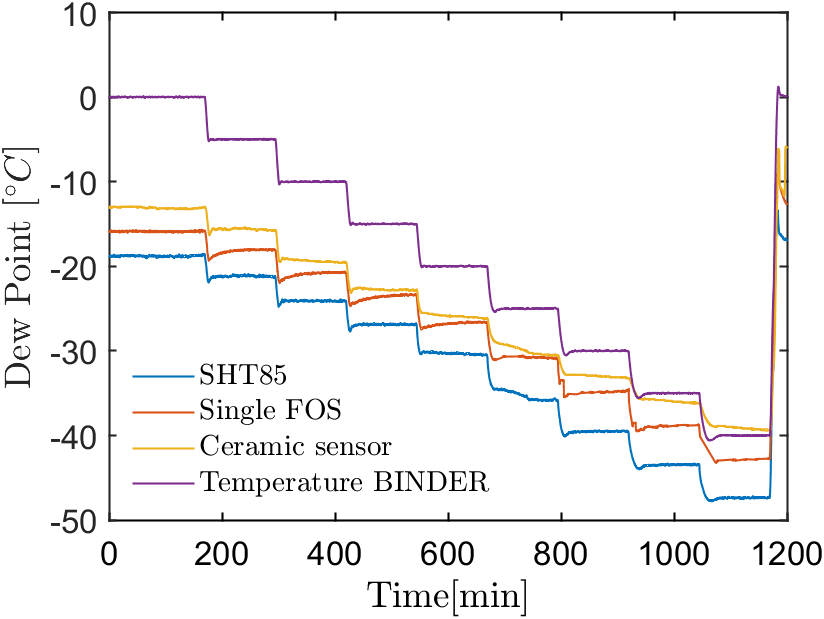
\includegraphics[width=0.6\columnwidth]{Chapter5/images/DPCPercent.png}
\caption{Comparison of the dew points calculated using the Magnus formula for the industrial sensor SHT85, metal oxide trace humidity sensor, and the hygrometer. For the comparison, the temperature inside the Binder climatic chamber was also plotted.}
\label{fig_comparison}
\end{figure}
The response of the hygrometer was also compared with the sniffing system and different lengths of the guidelines leading to the ceramic sensor. In the case of the \gls{STS} the sniffing system's electronic circuitry will be placed at least \SI{20}{\metre} away from the detector. For the plot depicted on the left side, the pipe was \SI{2}{\metre} and for the right one \SI{12}{\metre}, the time response was $1.5$~min and $3$~m. Assuming that the flow doesn't depend on the distance from the sniffing point, if the pipe was $30$~m the response would be $5.7$~min. 
\begin{figure}[!h]
\centering
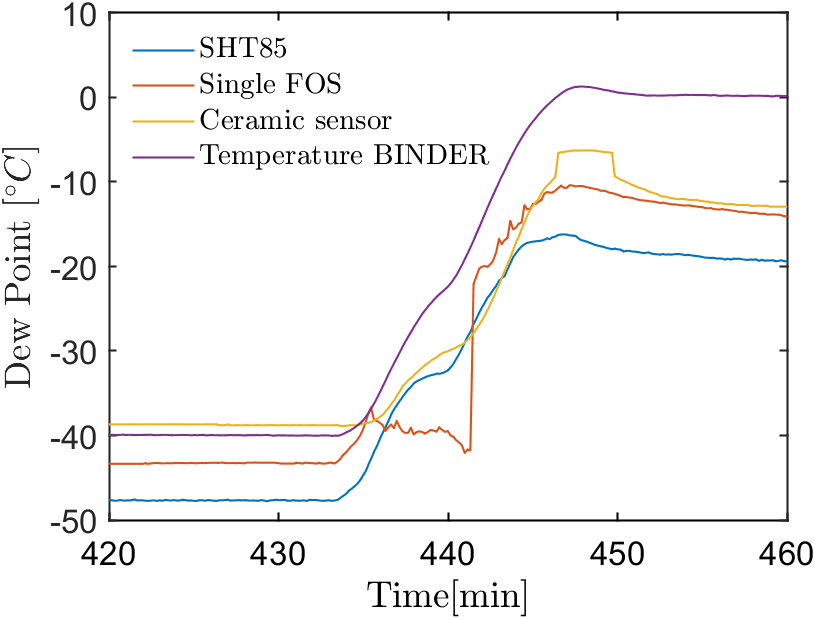
\includegraphics[width=0.47\columnwidth]{Chapter5/images/DPCPercent_response2m.png}
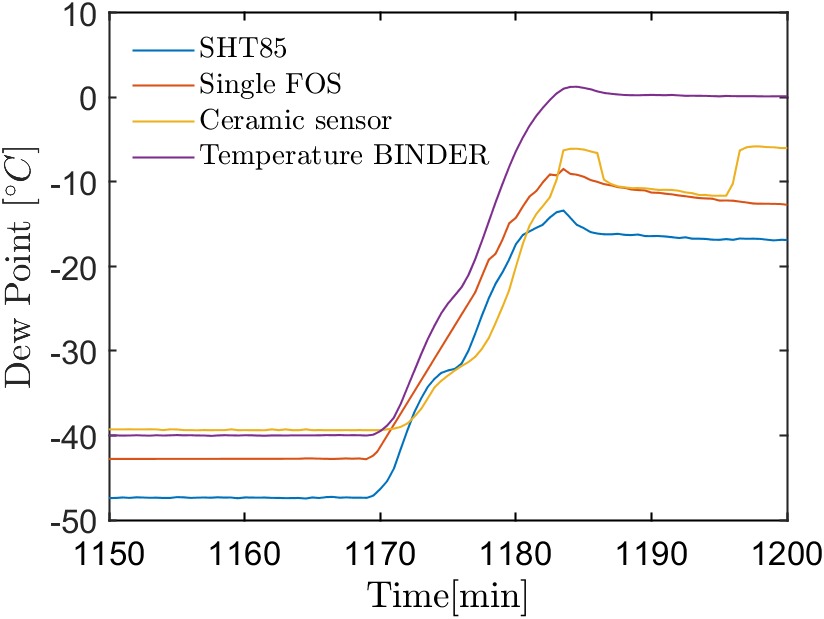
\includegraphics[width=0.47\columnwidth]{Chapter5/images/DPCPercent_response12m.png}
\caption{Time response comparison of different sensors. Left - \SI{2}{\metre} pipe to the ceramic sensors, right - \SI{12}{\metre} pipe to the ceramic sensors.}
\label{fig_comparison_hw}
\end{figure}
\newpage
Figure \ref{Tfig_comparison_2} shows the behavior of the fiber optic hygrometer at low dew points. The sensing limits are clearly represented in Figure~\ref{Tfig_comparison_2} with a red rectangle. Considering the area with a high point density, the limitations of the hygrometer could be assumed to be a dew point of \SI{-70}{\celsius}. But in that area, the uncertainties become much higher. It's also noteworthy that that limit refers to the measuring temperature of \SI{10}{\celsius}. On the other hand, for the dew points measured at \SI{20}{\celsius} the range shrinks to values of about \SI{-50}{\celsius}/\SI{-40}{\celsius}.

\begin{figure}[!h]
\centering
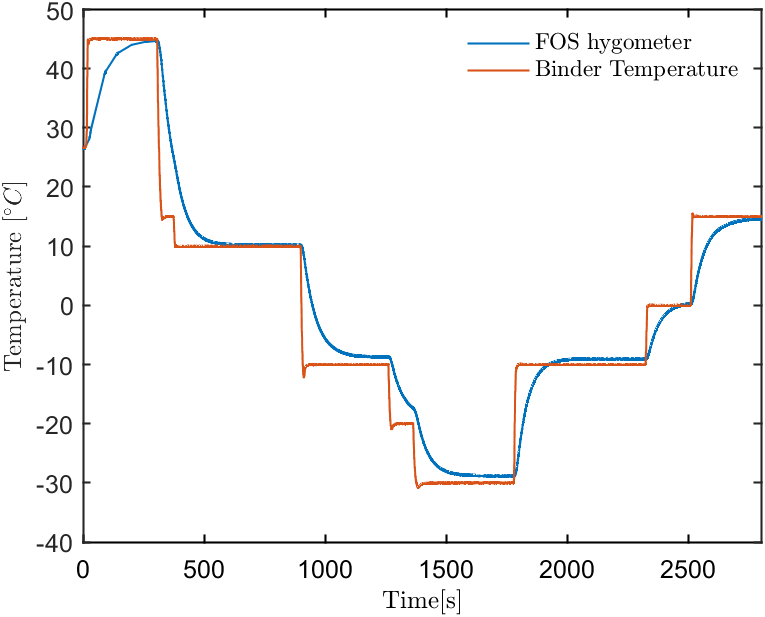
\includegraphics[width=0.47\columnwidth]{Chapter5/images/FOS_performance_T.png}
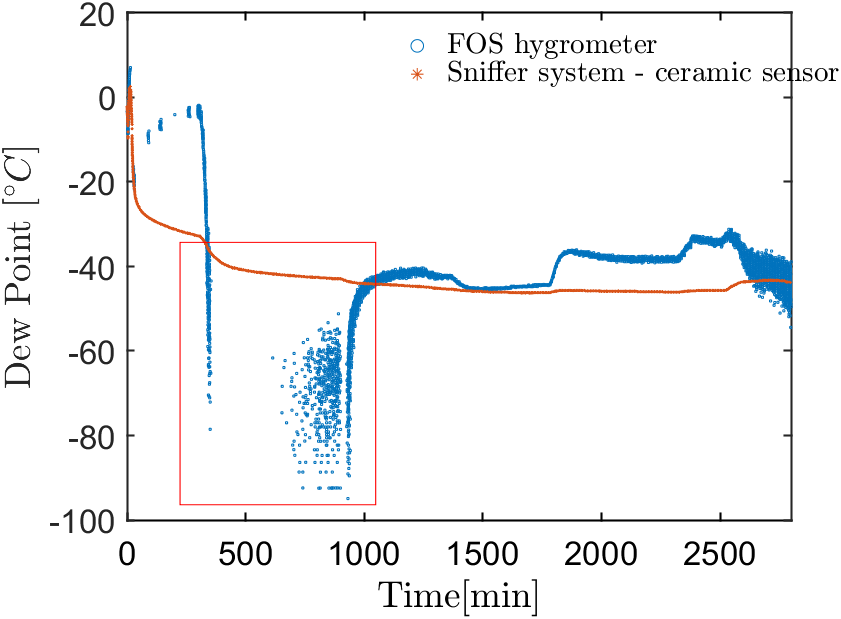
\includegraphics[width=0.47\columnwidth]{Chapter5/images/FOS_performance1.png}
\caption{The temperature inside the BINDER chamber and temperature measured by the hygrometer(left). Dew point during the changing ambient conditions per the hygrometer and the ceramic sensor.}
\label{Tfig_comparison_2}
\end{figure}
\section{Final considerations}
The characterization of the \gls{FOS} pointed out the advantages and limits of this particular technology with the use of polyimide as the sensitive material. In principle, the tested hygrometer meets the requirements set for the \gls{STS}. The distributed system could be also based on the \gls{FOS}. An array of sensors could be still considered, but the distance between the gratings should be much larger than \SI{15}{\cm} to ensure that the sensors can be put inside packaging in strain-free conditions. As mentioned in the section~\ref{fos_irrad}, the \gls{FBG} based \gls{FOS} can be considered radiation hard. According to Berutti~\cite{Berruti}, the sensors can be used in radiation environments by pre-irradiating them before installation, to reduce radiation-induced cross-sensitivity. 

Moreover, the capacitive industrial sensors will be used next to the \gls{FOS}. The main purpose will be to use them during the commissioning and in order to recalibrate the \gls{FOS} if the installation will cause any additional stress on the grating.

The last technology foreseen for the distributed sensing system is the metal oxide moisture sensor, which is a very reliable solution that will be used also for the interlocking system.  Several sniffing points inside the detector enclosure will also measure trace humidity and serve as a reference for the two other measurement technologies.